%%%%%%%%%%%%%%%%%%%%%%%%%%%%%%%%%%%%%%%%%%%%%%%%%%%%%%%%%%%%%%%
%
% Welcome to Overleaf --- just edit your LaTeX on the left,
% and we'll compile it for you on the right. If you open the
% 'Share' menu, you can invite other users to edit at the same
% time. See www.overleaf.com/learn for more info. Enjoy!
%
%%%%%%%%%%%%%%%%%%%%%%%%%%%%%%%%%%%%%%%%%%%%%%%%%%%%%%%%%%%%%%%
\documentclass{beamer}
\usetheme{Madrid}
\usecolortheme{seahorse}

\usepackage[linesnumbered,lined,boxed,commentsnumbered]{algorithm2e}

%%% Работа с русским языком и шрифтами
\usepackage{multicol}
\usepackage[english,russian]{babel}   % загружает пакет многоязыковой вёрстки
% \usepackage{fontspec}      % подготавливает загрузку шрифтов Open Type, True Type и др.
% \setmainfont[Ligatures={TeX,Historic}]{Myriad Pro} 
% \setsansfont{Myriad Pro}  
% \setmonofont{Courier New}
\uselanguage{russian}
\languagepath{russian}
\deftranslation[to=russian]{Theorem}{Теорема}
\deftranslation[to=russian]{Definition}{Определение}
\deftranslation[to=russian]{Definitions}{Определения}
\deftranslation[to=russian]{Corollary}{Следствие}
\deftranslation[to=russian]{Fact}{Факт}
\deftranslation[to=russian]{Example}{Пример}
\deftranslation[to=russian]{Examples}{Примеры}

\graphicspath{{images/}} 

\let\eps\varepsilon
\let\tab\indent 
\let\inf\infty  % colision with infinum
\let\alp\alpha 

\newcommand{\expect}{\mathsf{E}}
\newcommand{\disp}{\mathsf{D}}

\newcommand{\N}{\mathbb{N}}
\newcommand{\Z}{\mathbb{Z}}
\newcommand{\R}{\mathbb{R}}
\newcommand{\CC}{\mathbb{C}}
\newcommand{\Q}{\mathbb{Q}}
\newcommand{\Real}{\mathrm{Re}}
\newcommand{\supp}{\mathrm{supp}}

\DeclareMathOperator{\im}{Im}
\DeclareMathOperator{\marg}{arg}
\DeclareMathOperator{\Arg}{Arg}

\DeclareMathOperator{\sign}{sgn}

\newcommand{\abs}[1]{\left|{#1}\right|}
\newcommand{\limit}[2][\infty]{\displaystyle{\lim_{{#2} \to {#1}}}\ }
\newcommand{\limitu}[1]{\displaystyle{\varlimsup_{{#1} \to \infty}}}
\newcommand*{\dlim}[2]{\underset{y \to #2}{\lim\limits_{x \to #1}}}
\newcommand{\mysum}[2]{\displaystyle{\sum^{#1}_{#2}}}
\newcommand{\answer}[1]{\\\fbox{Ответ: $\displaystyle{} {#1}$.}}
\newcommand{\Mod}[1]{\ \mathrm{mod}\ #1}
\newcommand{\seq}{\ \underset{\text{сх.}}{\sim} \ }

\newcommand{\bline}{ \noindent\makebox[\linewidth]{\rule{\paperwidth}{0.4pt}}}
\newcommand{\aliq}{\mathrel{\raisebox{-0.2ex}{\vdots}}}

\renewcommand{\d}[1]{\,d#1}
\newcommand{\prt}[2]{\frac{\partial{#1}}{\partial{#2}}}
\newcommand{\pprt}[2]{\frac{\partial^2{#1}}{\partial{#2}^2}}

\newenvironment{exercise}[2][Задача]{\begin{trivlist} 
\item[\hskip \labelsep {\bfseries #1}\hskip \labelsep {\bfseries #2.}]}{\end{trivlist}}

\everymath{\displaystyle}

\newcommand{\imp}[1]{\textit{\color{blue}#1}}

\newcommand{\uneq}[1]{\ \underset{#1}{=}\ }
\newcommand{\skipline}[0]{$ $\\}


\title{Графы в машинном обучении}
\author[Романов Владимир]{Романов Владимир БПМИ192}
\institute[ВШЭ]{Национальный исследовательский университет \\ «Высшая школа экономики» (Москва)}
\date{23 ноября 2021 г.}

\begin{document}

\frame{\titlepage}

% \begin{frame}
%     \frametitle{Какие задачи на графы нам интересны?}
%     Задачи на вершины

%     \begin{itemize}
%         \item link-prediction
%         \item node-classification
%     \end{itemize}
%     \skipline
%     Задачи на графы

%     \begin{itemize}
%         \item graph-classification
%     \end{itemize}
% \end{frame}


\begin{frame}
    \frametitle{Vertex embeddings}
    \begin{block}{Определение}
        First-order proximity --- непосредственная близость вершин 
        \skipline
        \skipline
        Second-order proximity --- близость вершин по структуре
    \end{block}
    \skipline
    \begin{itemize}
        \item Рассмотрим embedding, которые описывают локальные свойства
        \item Мы хотим, чтобы соседи имели близкий вектор, а далекие разный
    \end{itemize}
    \skipline
    \skipline
    \skipline
    \begin{itemize}
        \item Формулировка напоминает аналогичную задачу для текста
        \item Идея: попытаемся применить SkipGram для этой задачи
    \end{itemize}
\end{frame}

\begin{frame}
    \frametitle{DeepWalk (Постановка)}

    \begin{block}{Обозначения}
        Embedding: $\varPhi: V \to \R^d$ 
        \skipline
        \skipline
        Loss: $\sum_{u \in N(v)} -\ln Pr\left(u \ \vert\ \varPhi(v)\right)$
    \end{block}
    \skipline
    \begin{block}{Алгоритм}
        \begin{enumerate}
            \item Переберем вершину $s \in V$
            \item Рассмотрим случайный путь $\mathcal{W}_s$ размера $t$
            \item Прорелаксируем SkipGram пройдясь по $\mathcal{W}_s$ окном $w$
            \item Повторим процес $\gamma$ раз
        \end{enumerate}
    \end{block}
\end{frame}


\begin{frame}
    \frametitle{DeepWalk (in a nutshell)}
    \begin{figure}
        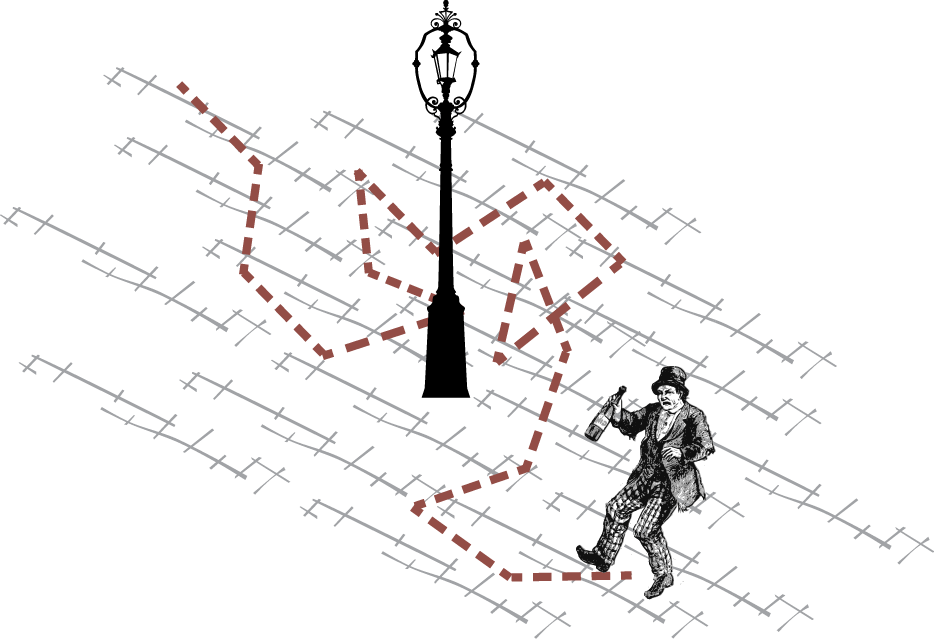
\includegraphics[width=1\columnwidth]{randomwalk.png}
    \end{figure}
\end{frame}

\begin{frame}
    \frametitle{DeepWalk (Hierarchical Softmax)}
    Проблема: делать Softmax долго
    \skipline
    % \skipline
    Решение: дерево отрезков \text{\color{blue} (или negative sampling)}
    \skipline
    \skipline
    $ $\hspace*{4ex} 
    $
    Pr\left(u \ \vert\ \varPhi(v)\right) = 
    \prod_{b_i \in B} Pr\left(b_i \ \vert\ \varPhi(v)\right)
    $ 
    \skipline
    \skipline
    \skipline
    Итоговый алгоритм:
    \begin{figure}
        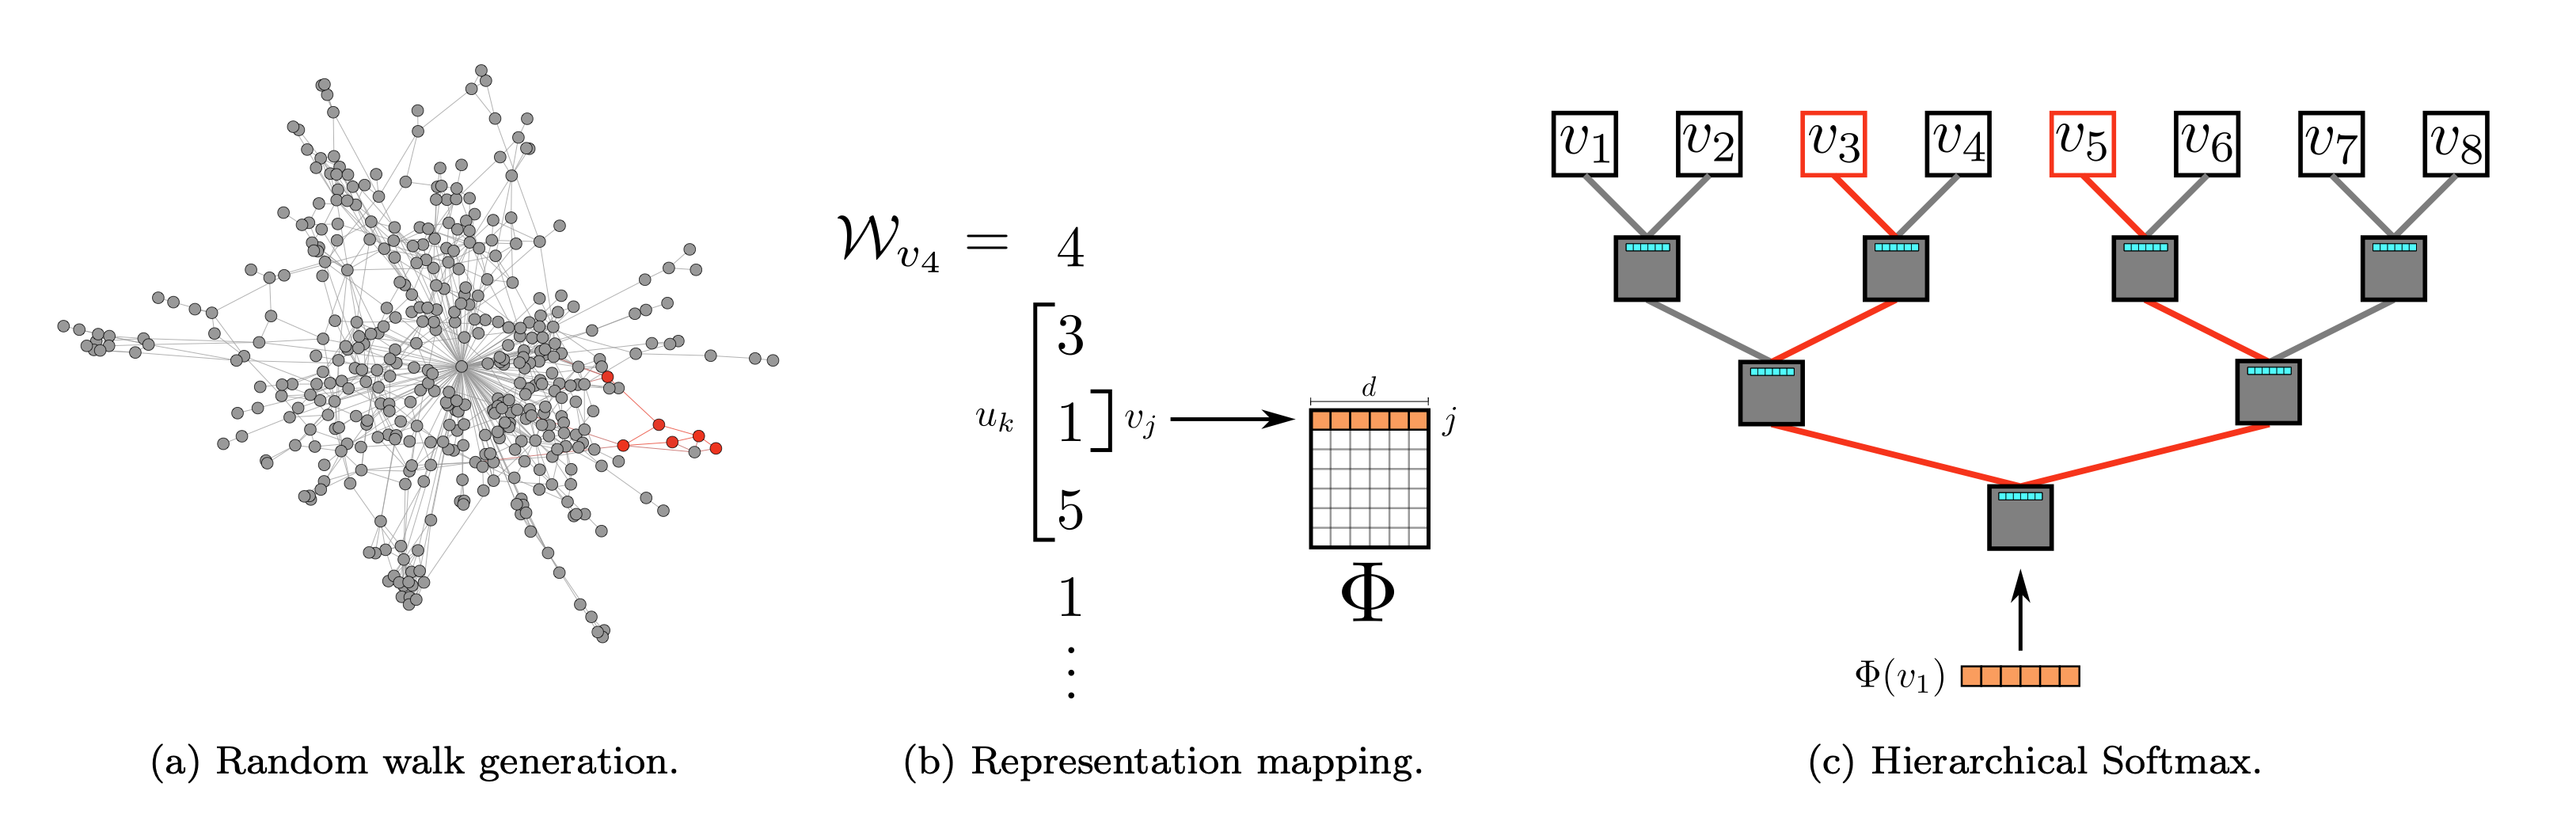
\includegraphics[width=1\columnwidth]{DeepWalk.png}
    \end{figure}
\end{frame}

\begin{frame}
    \frametitle{Node2Vec (search strategy)}
    \begin{block}{Обновление}
        Loss: $\sum_{u \in N_S  (v)} -\ln Pr\left(u \ \vert\ \varPhi(v)\right)$
    \end{block}
    \skipline
    \begin{multicols}{2}
        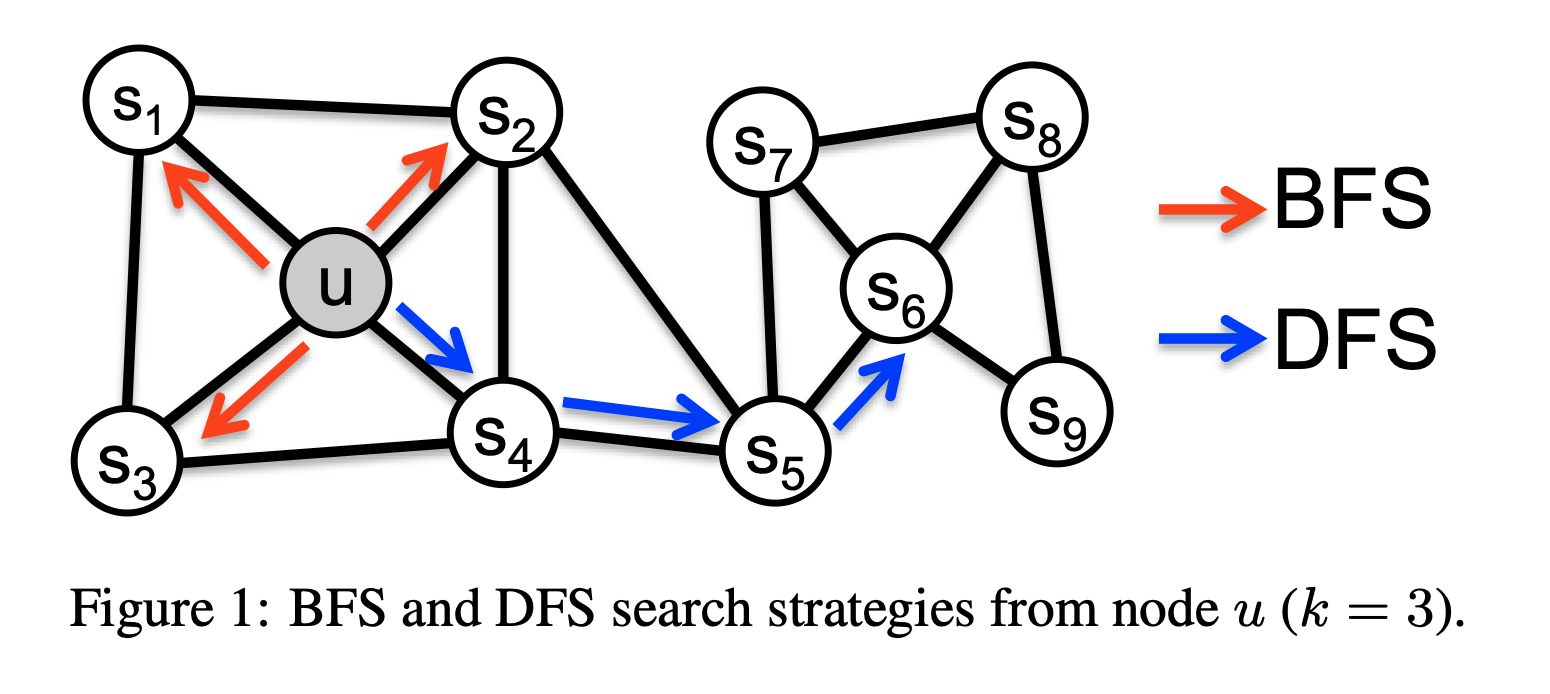
\includegraphics[width=1\columnwidth]{bfs_dfs.png}\par 
        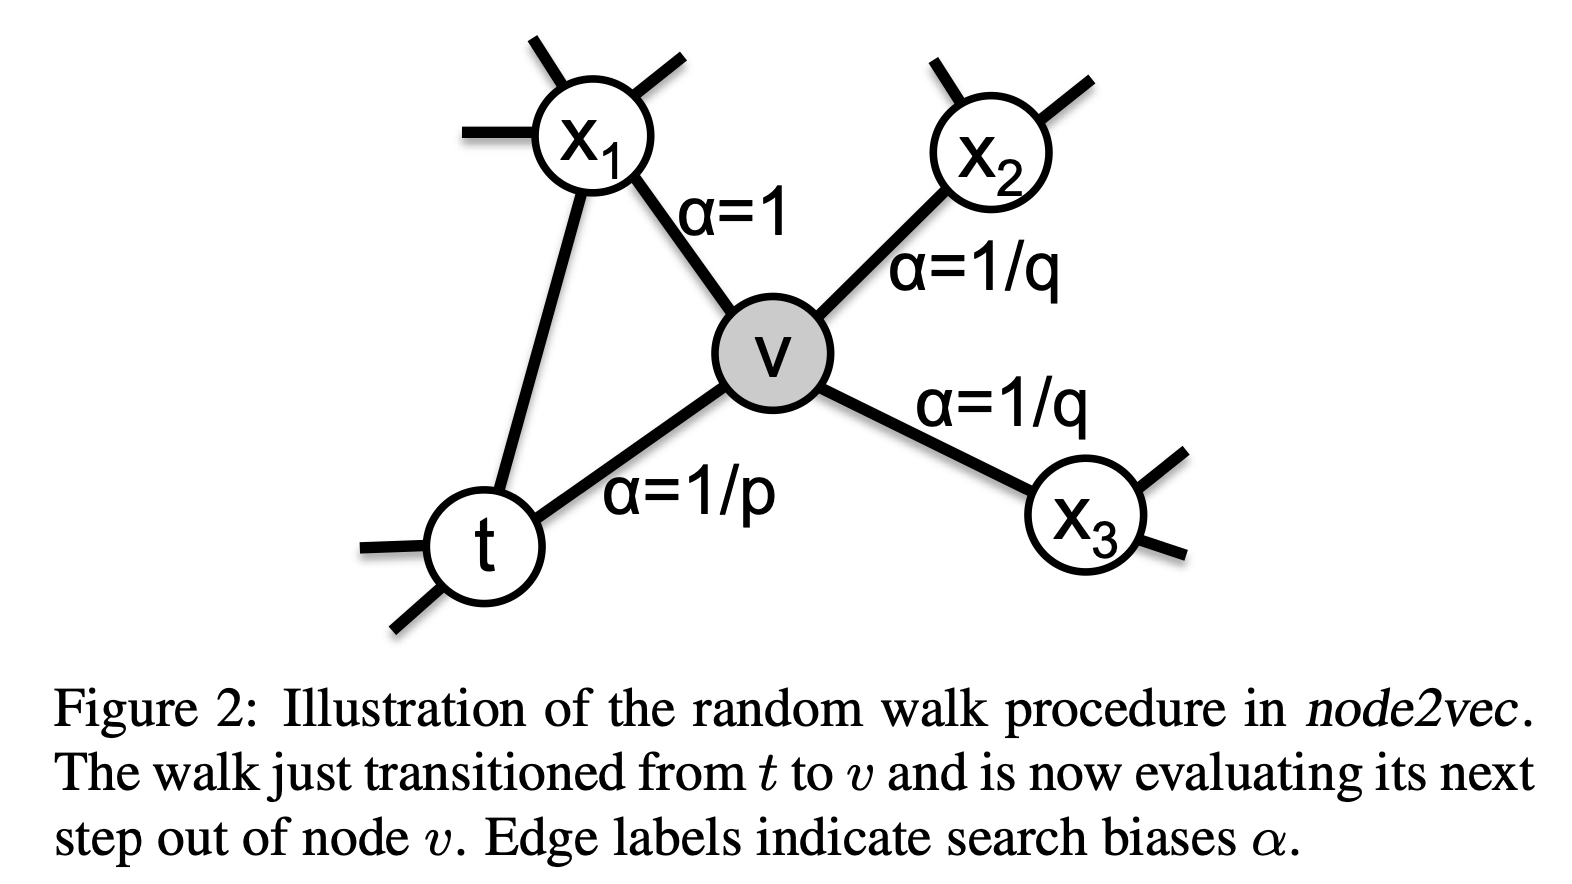
\includegraphics[width=1\columnwidth]{step.png}\par 
    \end{multicols}
\end{frame}

\begin{frame}
    \frametitle{Node2Vec (proximity)}
    Примеры кластеризации с разными параметрами $q$
    \begin{multicols}{2}
        \begin{figure}
            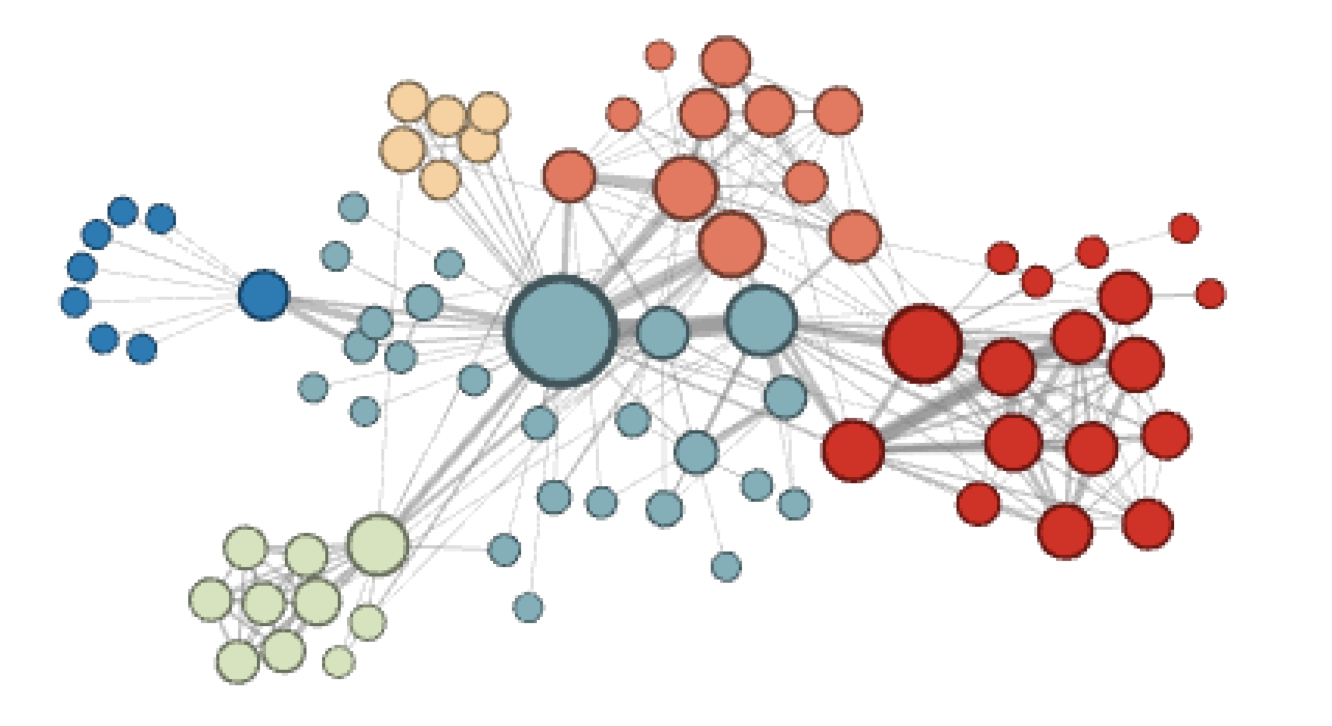
\includegraphics[width=1\columnwidth]{q_0_5.png}
            \caption{$p = 1, q = 0.5$}
        \end{figure}
        \par 
        \begin{figure}
            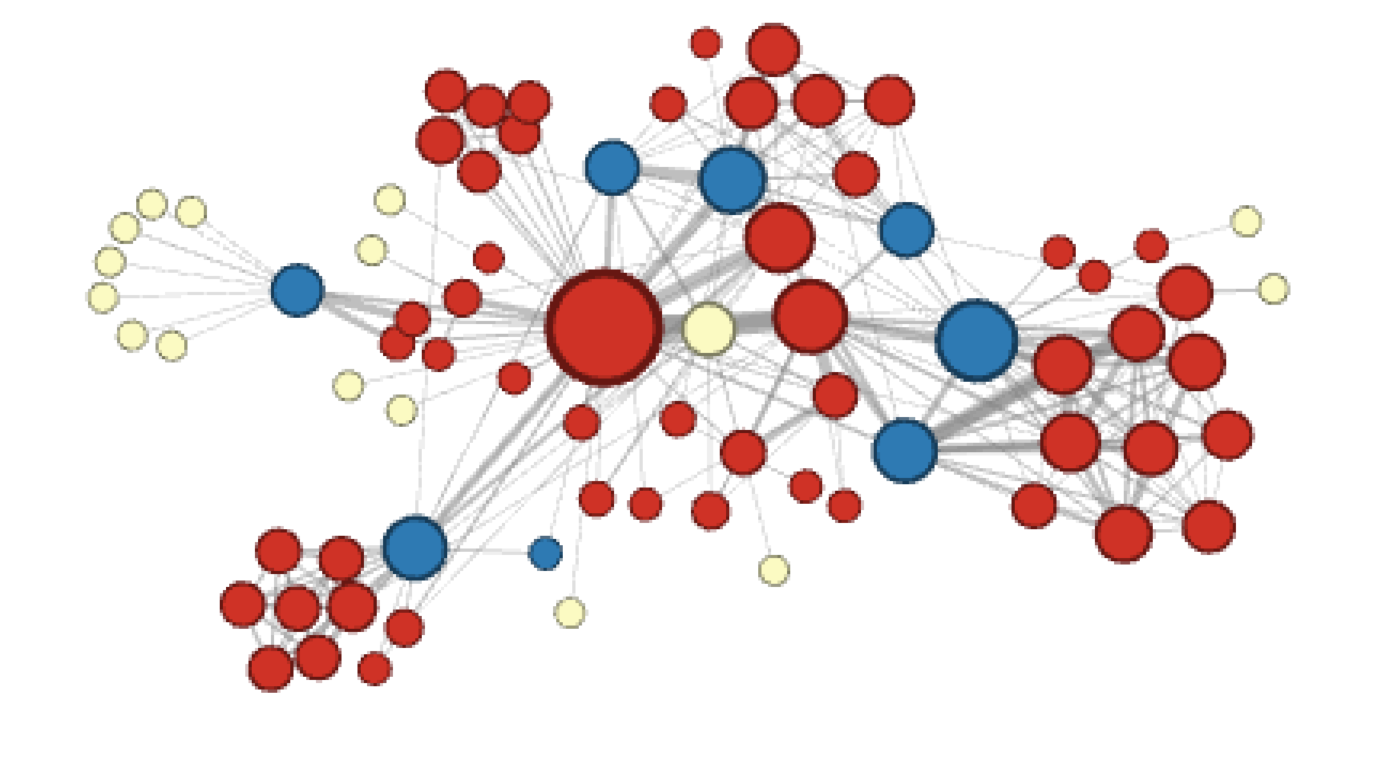
\includegraphics[width=1\columnwidth]{q_2.png}
            \caption{$p = 1, q = 2$}
        \end{figure}
        \par
    \end{multicols}
\end{frame}

\begin{frame}
    \frametitle{Structural Deep Network Embedding (SDNE)}
    Хотим в embedding также <<хранить>> знания о структуре\\ (second-order proximity)
    \begin{figure}
        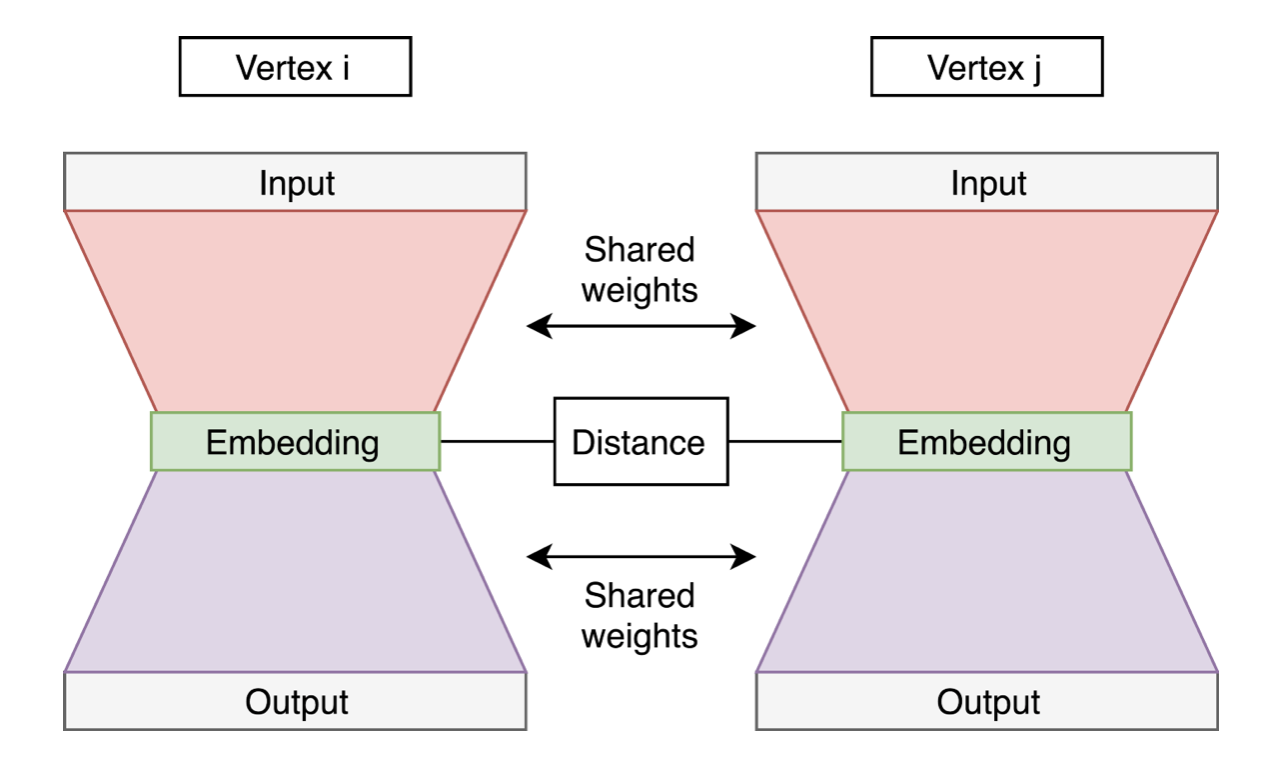
\includegraphics[width=0.75\columnwidth]{SDNE.png}
    \end{figure}
\end{frame}

\begin{frame}
    \frametitle{Какие задачи мы можем решить?}
    Возможные формулы оценки:
    \begin{figure}
        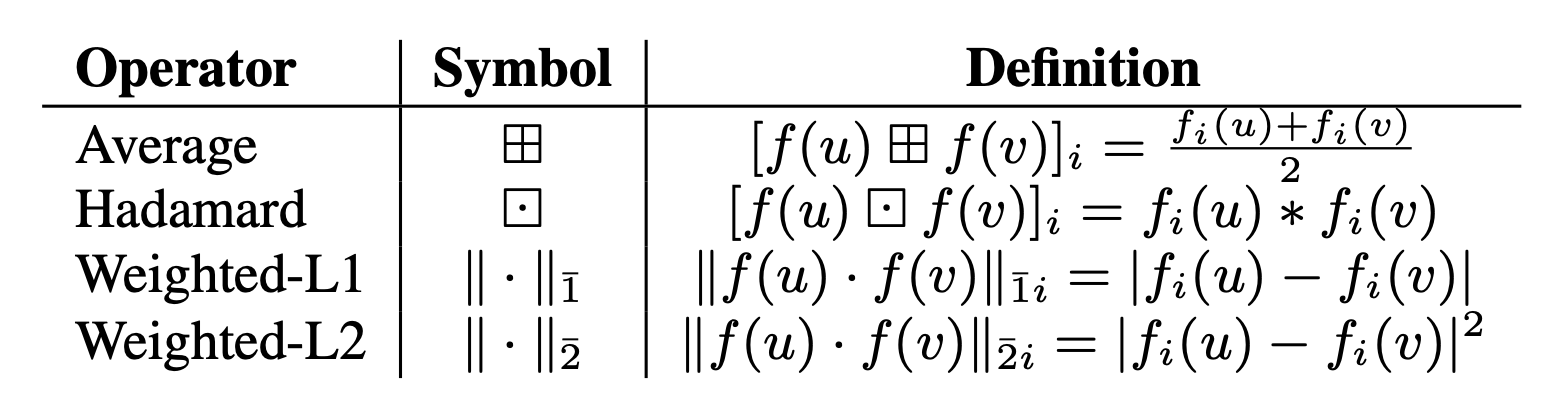
\includegraphics[width=0.75\columnwidth]{operators.png}
    \end{figure}
    \skipline
    Примеры задач:
    \begin{itemize}
        \item node-classification
        \item node-clastering
        \item graph-visualization
        \item link-prediction 
    \end{itemize}
\end{frame}

\begin{frame}
    \frametitle{Усложнение link-prediction}
    Постановка:
    \begin{itemize}
        \item Есть граф $\left(V, E\right)$
        \item Каждое ребро принадлежит одному из классов $(R)$
        \item Хотим найти $\phi(v_1, r, v_2)$, которая будет предсказывать, есть ли ребро $(v_1, v_2)$ класса $r$
    \end{itemize}
    \skipline
    Мы хотим предсказать трехмерный бинарный тензор $\R^{|V| \times |E| \times |V|}$
\end{frame}

\begin{frame}
    \frametitle{TuckER (decomposition)}
    \begin{figure}
        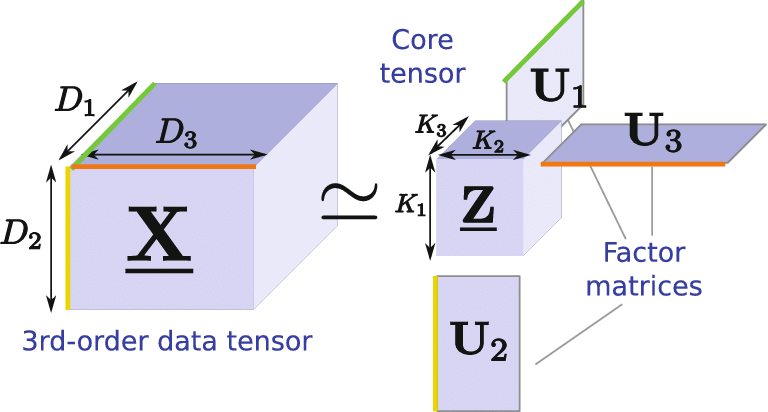
\includegraphics[width=0.6\columnwidth]{Tucker-decomposition.png}
    \end{figure}
    $$
    X_{ijk} = \sum_{\alpha=1}^{K_1} \sum_{\beta=1}^{K_2} \sum_{\gamma=1}^{K_3} 
    Z_{\alpha\beta\gamma} U^{(1)}_{i \alpha} U^{(2)}_{j \beta} U^{(3)}_{k \gamma} 
    $$
\end{frame}

\begin{frame}
    \frametitle{TuckER (model)}
    \begin{itemize}
        \item Попытаемся воспользоваться полученными embeddings для вершин
        \skipline
        \skipline
        \item Первая идея: обучить модель для каждого класса
        \skipline
        \skipline
        \item Вторая идея: обучим для классов свои embeddings, параллельно обучая ядро свертки
    \end{itemize}
\end{frame}

\begin{frame}
    \frametitle{TuckER (model)}
    \begin{figure}
        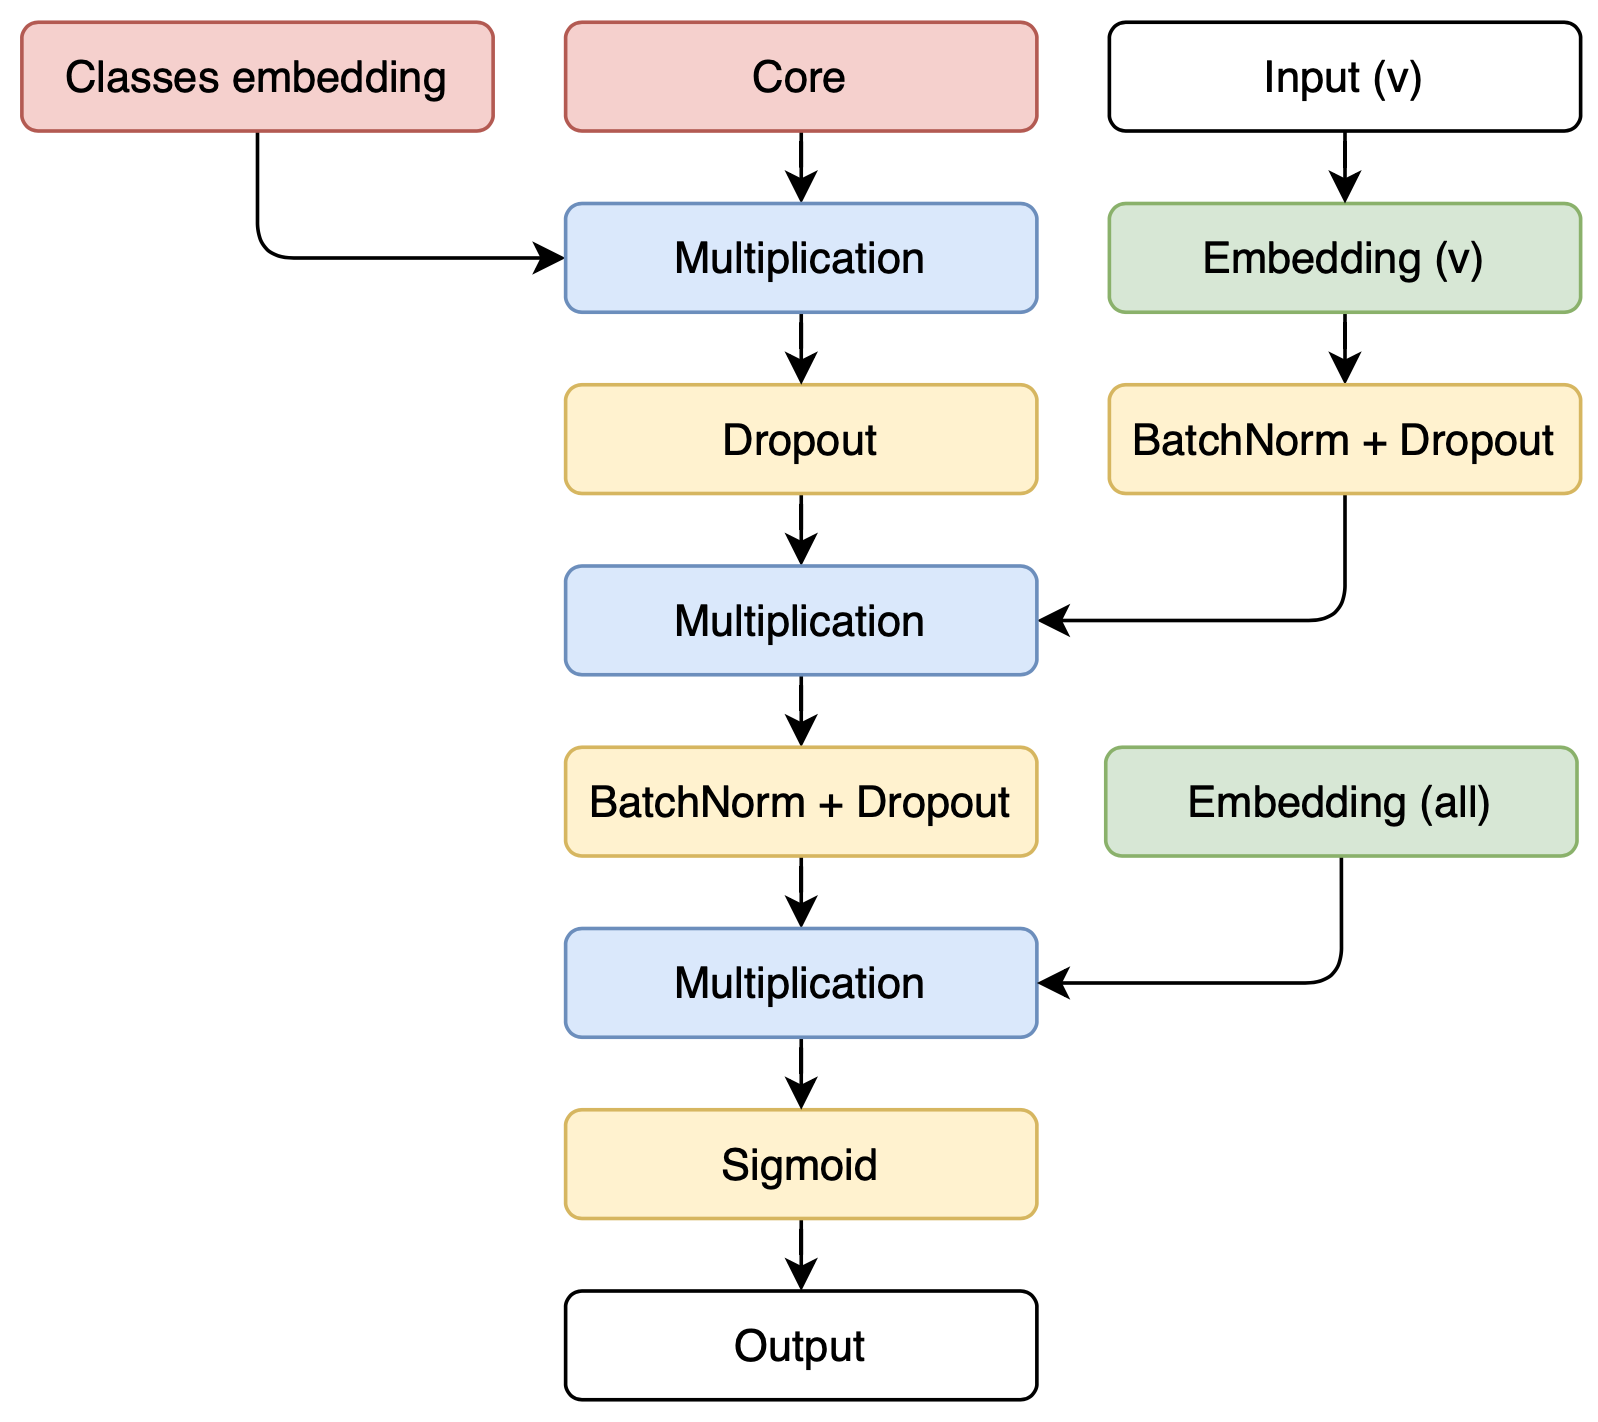
\includegraphics[width=0.7\columnwidth]{Diagram.png}
    \end{figure}
\end{frame}

\begin{frame}
\frametitle{Список литературы}
\begin{itemize}
    \item DeepWalk: \url{https://arxiv.org/pdf/1403.6652.pdf}
    \item Node2Vec: \url{https://arxiv.org/pdf/1607.00653.pdf}
    \item SDNE: \url{https://www.kdd.org/kdd2016/papers/files/rfp0191-wangAemb.pdf}
    \item TuckER: \url{https://arxiv.org/pdf/1901.09590.pdf}
\end{itemize}
\end{frame}


\end{document}